% --- Conteúdo ATUALIZADO para Tabela&Grafico/bubble_sort.tex ---

\qquad A seguir são apresentados os resultados obtidos na execução do algoritmo \textit{Bubble Sort}.

% --- IMAGEM DA TABELA DO BUBBLE SORT ---
\begin{figure}[h!]
    \centering
    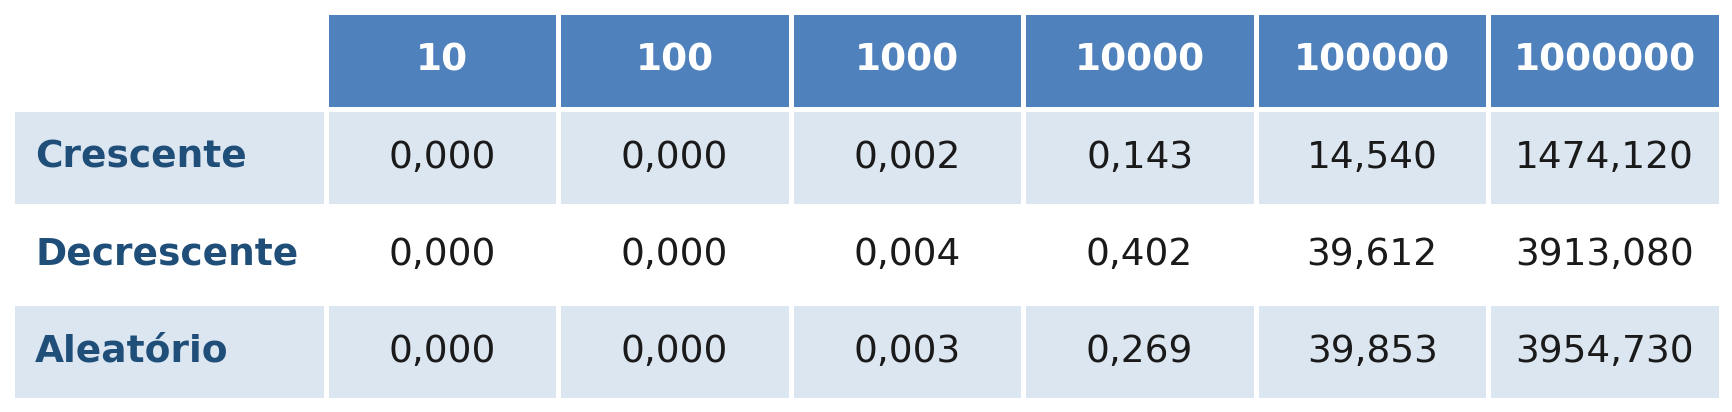
\includegraphics[width=1.0\textwidth]{Imagens/Bubble Sort/tabela_bubble.png}
    \caption{Tabela de tempo de execução (em segundos) do \textit{Bubble Sort} (elaborado pelo autor).}
    \label{fig:tabela_bubble}
\end{figure}

% --- IMAGEM DO GRÁFICO DO BUBBLE SORT ---
\begin{figure}[h!]
    \centering
    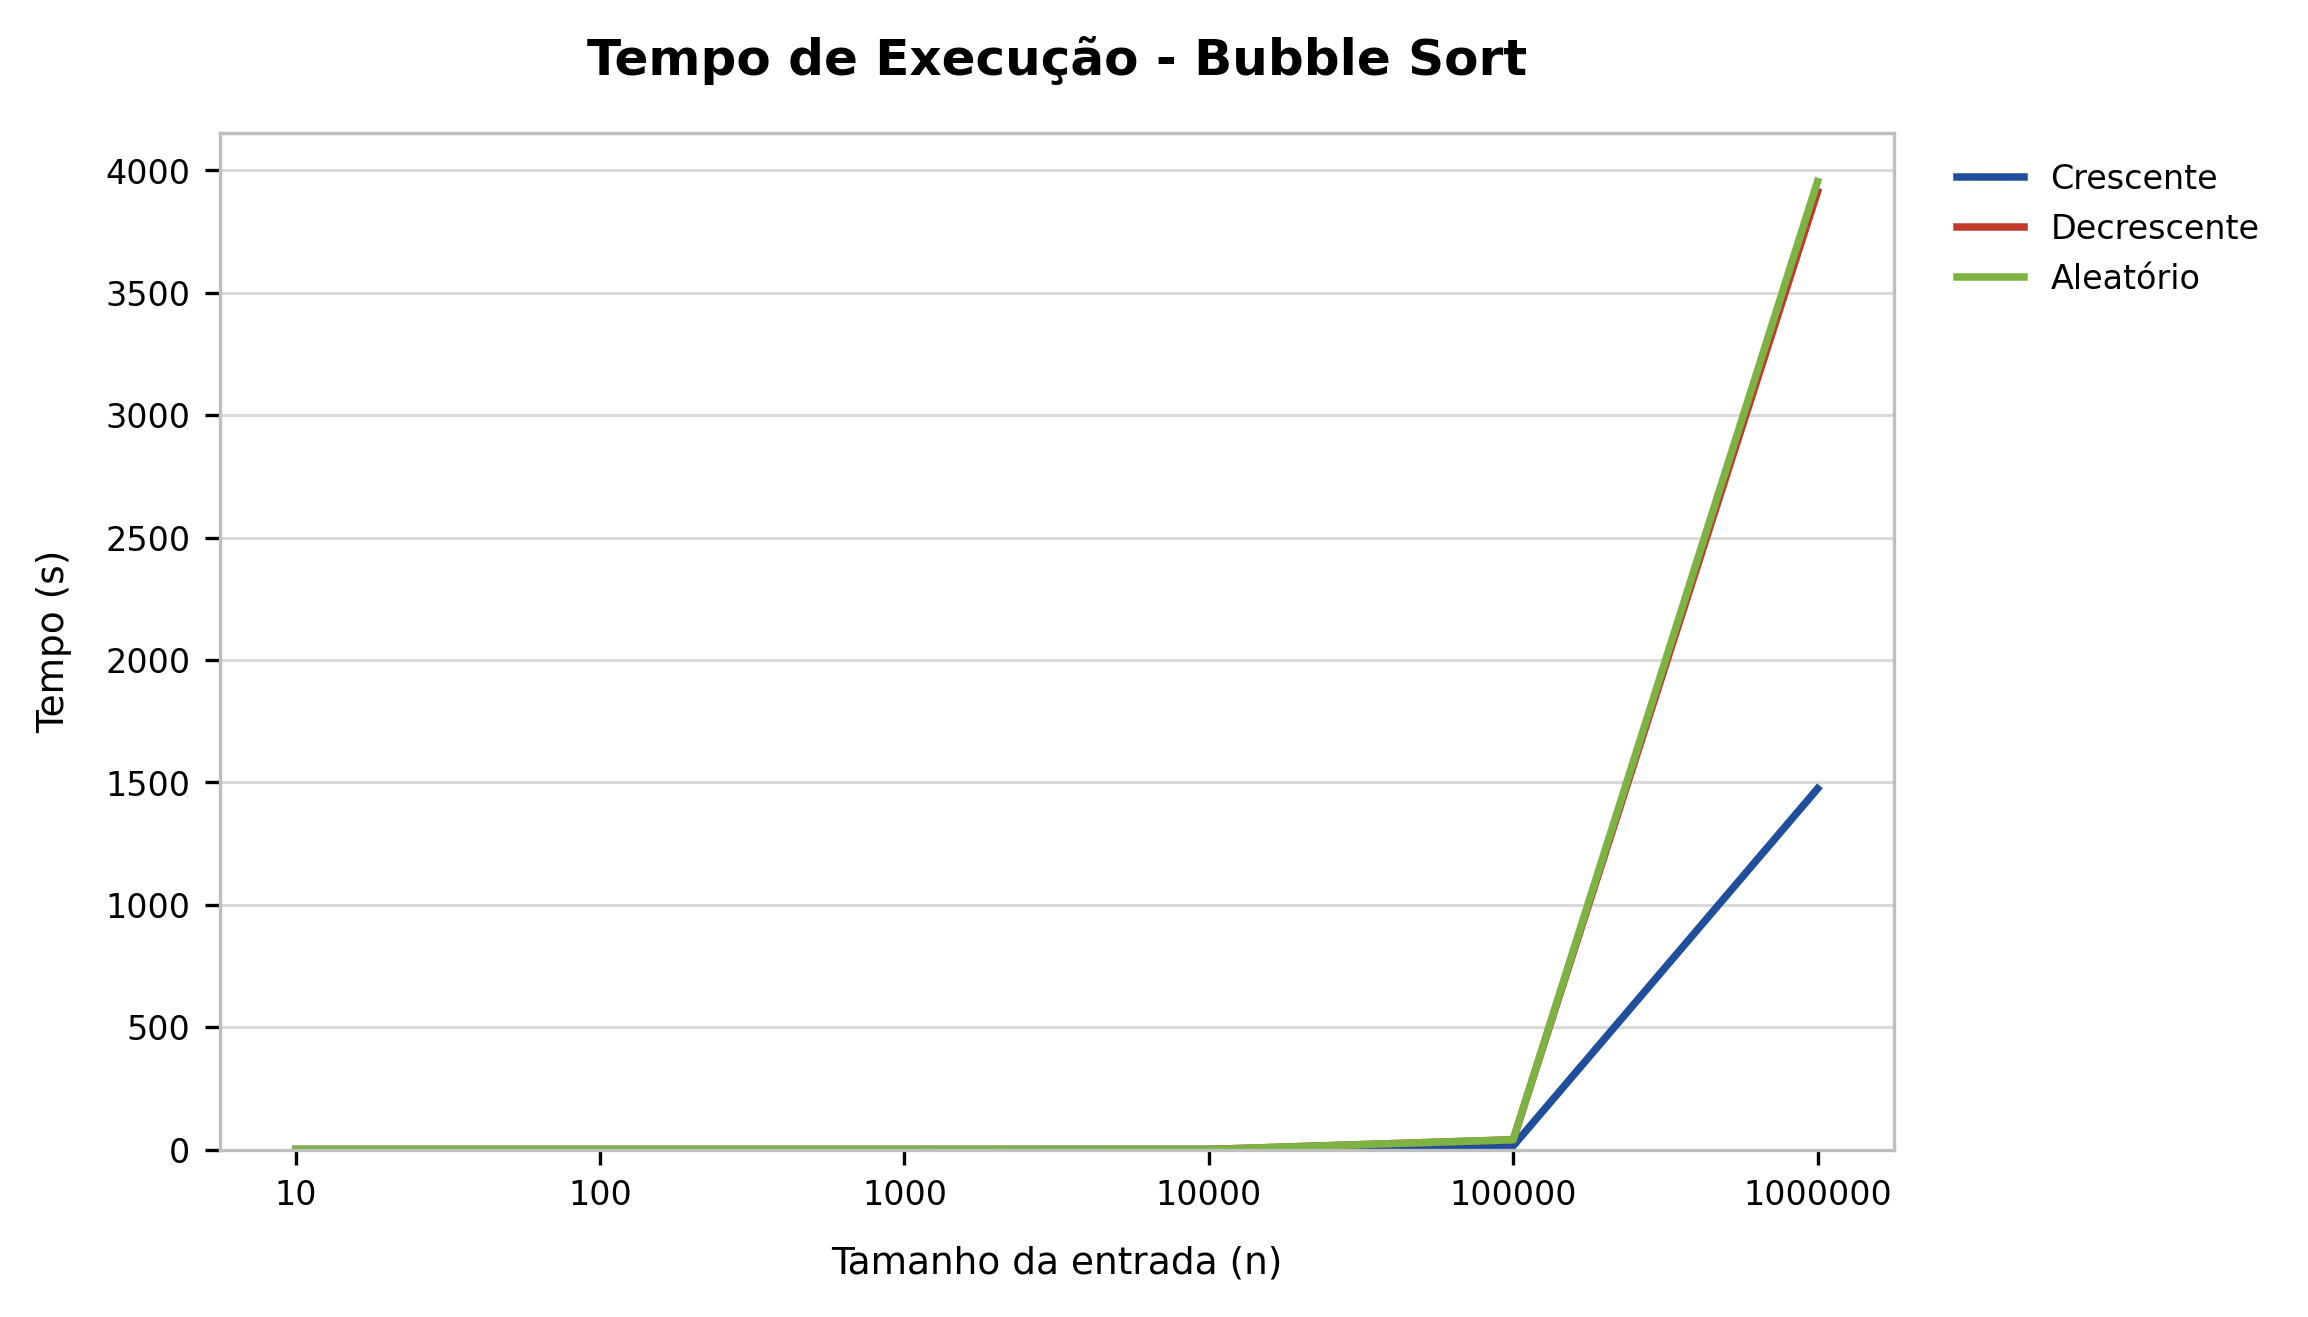
\includegraphics[width=1.0\textwidth]{Imagens/Bubble Sort/grafico_bubble.png}
    \caption{Desempenho do Algoritmo \textit{Bubble Sort} (elaborado pelo autor).}
    \label{fig:grafico_bubble}
\end{figure}

% --- ANÁLISE DOS RESULTADOS DO BUBBLE SORT ---

\qquad Os dados da Figura \ref{fig:tabela_bubble} e o gráfico da Figura \ref{fig:grafico_bubble} mostram o comportamento quadrático esperado para o \textit{Bubble Sort}, com tempos que se tornam proibitivos em entradas grandes. Para as entradas de 10 e 100 elementos, os tempos registrados foram de 0,000 segundo em todos os cenários, o que indica apenas que a duração ficou abaixo da precisão do relógio utilizado.

\begin{itemize}
    \item \textbf{Crescente (melhor caso):} mesmo com o vetor já ordenado, a implementação utilizada não possui mecanismo de parada antecipada, de modo que os laços aninhados são percorridos por completo. O tempo para um milhão de elementos foi de 1.474,120 segundos (cerca de 25 minutos). A vantagem desse cenário vem apenas da ausência de trocas, já que o número de comparações é o mesmo dos demais casos.

    \item \textbf{Decrescente (pior caso):} é o cenário que exige o número máximo de trocas, uma para cada comparação realizada. O tempo para um milhão de elementos foi de 3.913,080 segundos (aproximadamente 1 hora e 5 minutos), cerca de 2,7 vezes maior que o do vetor crescente.

    \item \textbf{Aleatório (caso médio):} o tempo foi de 3.954,730 segundos (aproximadamente 1 hora e 6 minutos), praticamente igual ao do pior caso. Isso mostra que, na prática, o \textit{Bubble Sort} não obtém ganho relevante em entradas desordenadas.
\end{itemize}

\qquad Um resultado que merece atenção é o fato de o caso aleatório ter sido ligeiramente mais lento que o decrescente, tanto em $n = 100.000$ (39,853 s contra 39,612 s) quanto em $n = 1.000.000$ (3.954,730 s contra 3.913,080 s), contrariando à primeira vista a expectativa teórica. A explicação está na implementação utilizada: como não há parada antecipada, o número de comparações é idêntico nos três cenários, e apenas o número de trocas varia. No vetor decrescente todas as comparações resultam em troca, mas seguindo um padrão regular de acesso à memória; no vetor aleatório o padrão é irregular, o que aumenta os erros de previsão de desvio no processador. A diferença observada, inferior a 1\%, está dentro da variação esperada para medições em hardware real e não altera a classificação de complexidade.

\qquad De modo geral, os testes confirmam o comportamento $O(n^2)$ do \textit{Bubble Sort} em todos os cenários avaliados para a implementação utilizada, o que o torna inadequado para conjuntos de dados de grande porte.

\FloatBarrier